




%%%%%%%%%%%%%%%%%%%%%%%%%%%%%%%%%%%%%%%%%%%%%%%%%%%%%%%%%%%%%%%%%%%%%%%%%%%%%%%
\documentclass{article}
\newcommand{\path}{../../../assets/settings}
\input{\path/newcommand.tex}
\input{\path/usepackage.tex}


\usepackage{nopageno} % Paquete para desactivar la numeración de páginas

\begin{document}
%%%%%%%%%%%%%%%%%%%%%%%%%%%%%%%%%%%%%%%%%%%%%%%%%%%%%%%%%%%%%%%%%%%%%%%%%%%%%%%


\subsection{Perdidas por orientacion e inclinacion}


%%%%%%%%%%%%%%%%%%%%%%%%%%%%%%%%%%%%%%%%%%%%%%%%%%%%%%%%%%%%%%%%%%%%%%%%%%%%%
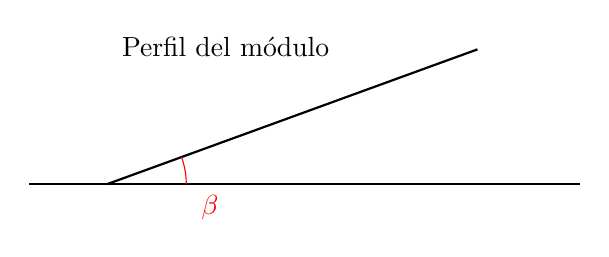
\begin{tikzpicture}

    \def\L{5} % Longitud de la recta
    \def\theta{20} % Ángulo de la recta en grados

    % Dibujar el suelo
    \draw[thick] (-1, 0) -- (6, 0) ;
    
    % Dibujar el módulo inclinado
    \draw[thick] (0, 0) -- ({\L*cos(\theta)}, {\L*sin(\theta)});
    
    % Dibujar el ángulo beta
    \draw[color=red] (1, 0) arc[start angle=0, end angle=\theta, radius=1];
    \node[color=red] at (1.3, -0.3) {$\beta$};
    
    % Añadir etiquetas y dimensiones
    \node[above] at (1.5, 1.5) {Perfil del módulo};
    
    \end{tikzpicture}
%%%%%%%%%%%%%%%%%%%%%%%%%%%%%%%%%%%%%%%%%%%%%%%%%%%%%%%%%%%%%%%%%%%%%%%%%%%%%


%%%%%%%%%%%%%%%%%%%%%%%%%%%%%%%%%%%%%%%%%%%%%%%%%%%%%%%%%%%%%%%%%%%%%%%%%%%%%
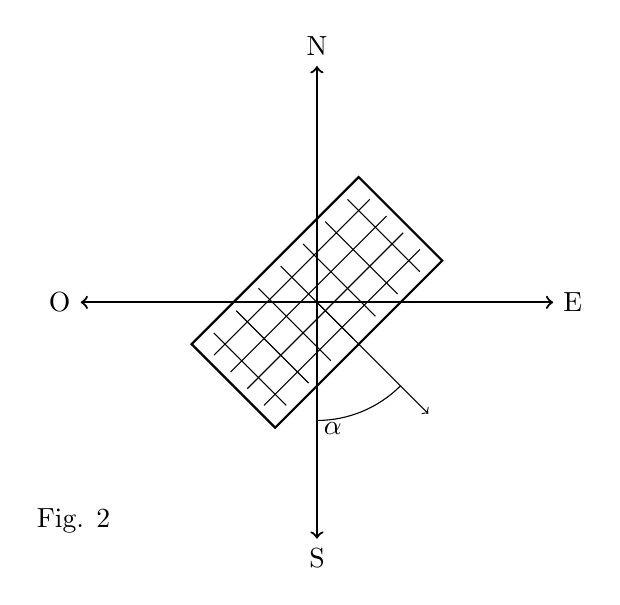
\begin{tikzpicture}

    % Dibujar las flechas de dirección
    \draw[thick, ->] (0, 0) -- (0, 3) node[above] {N}; % Flecha hacia el Norte
    \draw[thick, ->] (0, 0) -- (0, -3) node[below] {S}; % Flecha hacia el Sur
    \draw[thick, ->] (0, 0) -- (3, 0) node[right] {E}; % Flecha hacia el Este
    \draw[thick, ->] (0, 0) -- (-3, 0) node[left] {O}; % Flecha hacia el Oeste
    
    % Dibujar el teclado inclinado
    \begin{scope}[rotate=45]
        \draw[thick] (-1.5, -0.75) rectangle (1.5, 0.75);
        \foreach \x in {-1.2, -0.8, -0.4, 0, 0.4, 0.8, 1.2} {
            \draw (\x, -0.65) -- (\x, 0.65);
        }
        \foreach \y in {-0.45, -0.15, 0.15, 0.45} {
            \draw (-1.4, \y) -- (1.4, \y);
        }
    \end{scope}
    
    % Dibujar el ángulo alpha
    \draw[->] (0,0) -- (-90+45:2);
    
    \draw (0, -1.5) arc[start angle=-90, end angle=-90+45, radius=1.5];
    \node at (0.2, -1.6) {$\alpha$};
    
    % Añadir etiquetas y dimensiones
    \node[below left] at (-2.5, -2.5) {Fig. 2};
    
    \end{tikzpicture}
    %%%%%%%%%%%%%%%%%%%%%%%%%%%%%%%%%%%%%%%%%%%%%%%%%%%%%%%%%%%%%%%%%%%%%%%%%%%%%


    \ifdefined\inputado % para que no meta la bibliografia de los parciales al inclustarlo con input en otro
    \else
    \bibliographystyle{plainnat}
    \bibliography{\path/referencias}
    \fi
    

    \end{document}
